\documentclass{article}

\usepackage{fancyhdr}
\usepackage{extramarks}
\usepackage{amsmath}
\usepackage{amssymb}
\usepackage{amsthm}
\usepackage{amsfonts}
\usepackage{tikz}
\usepackage[plain]{algorithm}
\usepackage{algpseudocode}
\usepackage{lastpage}
\usepackage{caption}
\usepackage{subcaption}
\usepackage{nth}
\usetikzlibrary{automata,positioning,trees,dsp,chains,decorations.pathreplacing,angles,quotes,angles}
\usepackage[makeroom]{cancel}
\usepackage{mathtools}
\usepackage{listing}
\usepackage{color}
\usepackage[numbered,framed]{matlab-prettifier}
\usepackage{bold-extra}
\usepackage[T1]{fontenc} 
\usepackage{parskip}
\usepackage{gensymb}
\usepackage{siunitx}
\usepackage[nottoc,numbib]{tocbibind}
\usepackage[hidelinks]{hyperref}

%
% Basic Document Settings
%

% for figures: caption label is italic, the caption text is bold / italic
\captionsetup[figure]{labelfont=it,textfont={bf,it}}
% for subfigures: caption label is bold, the caption text normal.
% justification is raggedright (i.e. left aligned)
% singlelinecheck=off means that the justification setting is used even when the caption is only a single line long. 
% if singlelinecheck=on, then caption is always centered when the caption is only one line.
\captionsetup[subfigure]{labelfont=bf,textfont=normalfont,justification=raggedright,aboveskip=12pt}

\topmargin=-0.45in
\evensidemargin=0in
\oddsidemargin=0in
\textwidth=6.5in
\textheight=9.0in
\headsep=0.25in

\linespread{1.1}

\pagestyle{fancy}
\lhead{\hmwkAuthorName}
%\chead{\hmwkClass\ (\hmwkClassInstructor\hmwkClassTime): \hmwkTitle}
\chead{\hmwkClass\ : \hmwkTitle}
%\rhead{\firstxmark}
\rhead{\hmwkDueDate}
%\lfoot{\lastxmark}
\cfoot{\thepage\ of \pageref{LastPage}}

\renewcommand\headrulewidth{0.4pt}
\renewcommand\footrulewidth{0.4pt}

\setlength\parindent{0pt}

%
% Create Problem Sections
%

\newcommand{\enterProblemHeader}[1]{
    \nobreak\extramarks{}{Problem #1 continued on next page\ldots}\nobreak{}
    \nobreak\extramarks{Problem #1 (continued)}{Problem #1 continued on next page\ldots}\nobreak{}
}

\newcommand{\exitProblemHeader}[1]{
    \nobreak\extramarks{Problem #1 (continued)}{Problem #1 continued on next page\ldots}\nobreak{}
    \nobreak\extramarks{Problem #1}{}\nobreak{}
}

\newcounter{partCounter}
\nobreak\extramarks{Problem 1}{}\nobreak{}

%
% Homework Problem Environment
%
% This environment takes an optional argument. When given, it will adjust the
% problem counter. This is useful for when the problems given for your
% assignment aren't sequential. See the last 3 problems of this template for an
% example.
%
\newenvironment{homeworkProblem}[1][1]{
    \setcounter{secnumdepth}{0}
    \section{Problem #1}
    \enterProblemHeader{Problem #1}
}{
    \exitProblemHeader{\thesection}
}

%
% Homework Details
%   - Title
%   - Due date
%   - Due Time
%   - Class
%   - Section/Time
%   - Instructor
%   - Author
%

\newcommand{\hmwkTitle}{Problem Set Title}
\newcommand{\hmwkDueDate}{Due Date}
\newcommand{\hmwkClass}{Class Title}
\newcommand{\hmwkClassTime}{ 4:30 PM} % include a leading space if you choose to use this field (disabled for now)
\newcommand{\hmwkClassInstructor}{Instructor's Name} % (disabled for now)
\newcommand{\hmwkAuthorName}{\textbf{Student's Name}}

%
% Title Page
%


\title{
    \vspace{2in}
    \textmd{\textbf{\hmwkClass:\ \hmwkTitle}}\\
    \normalsize\vspace{0.1in}\small{Due\ on\ \hmwkDueDate}\\
    %\vspace{0.1in}\large{\textit{\hmwkClassInstructor\hmwkClassTime}}
    \vspace{2in}
}

\author{\hmwkAuthorName}
\date{}

\renewcommand{\part}[1]{\textbf{\large Part \Alph{partCounter}}\stepcounter{partCounter}\\}

%
% Various Helper Commands
%

% Useful for algorithms
\newcommand{\alg}[1]{\textsc{\bfseries \footnotesize #1}}

% For derivatives
\newcommand{\deriv}[1]{\frac{\mathrm{d}}{\mathrm{d}x} (#1)}

% For partial derivatives
\newcommand{\pderiv}[2]{\frac{\partial}{\partial #1} (#2)}

% Integral dx
\newcommand{\dx}{\mathrm{d}x}

% Alias for the Solution section header
\newcommand{\solution}{\textbf{\large Solution}}

% Probability commands: Expectation, Variance, Covariance, Bias
\newcommand{\E}[1]{\mathrm{E}\left\{#1\right\}}
\newcommand{\Var}[1]{\mathrm{Var}\left(#1\right)}
\newcommand{\Cov}[2]{\mathrm{Cov}\left(#1,#2\right)}
\newcommand{\Bias}{\mathrm{Bias}}

% Bayes Classifiers
\newcommand{\clsfr}[2]{\;\operatorname*{\gtrless}\limits_{\omega_{#1}}^{\omega_{#2}}\;}

% general
\newcommand{\logb}[2]{\mathit{log}_{#1}\left(#2\right)}
\newcommand{\code}[1]{\texttt{#1}}

% Transfer function commands
\newcommand{\z}[1]{#1(z)}
\newcommand{\ejw}[1]{#1(e^{j\omega})}
\newcommand{\ejO}[1]{#1(e^{j\Omega})}
\newcommand{\nz}[1]{z^{-#1}}
\newcommand{\ejp}[1]{e^{j#1}}
\newcommand{\ejn}[1]{e^{-j#1}}
\newcommand{\piover}[2]{\frac{#1\pi}{#2}}

% Discrete equations
\newcommand{\df}[1]{#1[n]}
\newcommand{\dfd}[2]{#1[n{-}#2]}
\newcommand{\dfn}[2]{#1[#2]}

% Array processing definitions
\newcommand{\kz}{k_{z}}

% Shortcuts for inter document references.
\newcommand{\lref}[1]{Listing \ref{#1} on page \pageref{#1}}
\newcommand{\eref}[1]{(\ref{#1})}
\newcommand{\fref}[1]{Figure \ref{#1}}
\newcommand{\tref}[1]{Table \ref{#1}}

% Matrices and Vectors
\newcommand{\mtx}[1]{\boldsymbol{#1}}
\newcommand{\mtxc}[1]{\boldsymbol{#1}^{*}}
\newcommand{\mtxh}[1]{\boldsymbol{#1}^{H}}
\newcommand{\mtxt}[1]{\boldsymbol{#1}^{T}}


% For more options see https://en.wikibooks.org/wiki/LaTeX/Source_Code_Listings
\lstset{
  style              = Matlab-editor,
  basicstyle         = \mlttfamily\footnotesize,
  escapechar         = ",
  mlshowsectionrules = true,
}

% When there are many figures it can take a long time to generate the document.
% Uncomment the following line skip generating any figures that are surrounded
% by '\ifx \skipfigures \defined' ... and '\fi'.
%\newcommand{\skipfigures}[0]{xxx}

\begin{document}

\maketitle
\pagebreak


%%%%%%%%%%%%%%%%%%%%%%%%%%%%%%%%%%%%%%%%%%%%%%%%%%%%
%%%%%%%%%%%%%%%%%%%%%%%%%%%%%%%%%%%%%%%%%%%%%%%%%%%%
%%%%%%%%%%%%%%%%%%%%%%%%%%%%%%%%%%%%%%%%%%%%%%%%%%%%
%%%%%%%%%%%%%%%%%%%%%%%%%%%%%%%%%%%%%%%%%%%%%%%%%%%%
\setcounter{secnumdepth}{0} % for sections that aren't HW problems include a counter reset so that section number doesn't appear
\section{Introduction}
\subsection{a)}
Introduction section that isn't numbered
\subsection{b)}
More introduction
\subsection{c)}
Even more introduction


%%%%%%%%%%%%%%%%%%%%%%%%%%%%%%%%%%%%%%%%%%%%%%%%%%%%
%%%%%%%%%%%%%%%%%%%%%%%%%%%%%%%%%%%%%%%%%%%%%%%%%%%%
%%%%%%%%%%%%%%%%%%%%%%%%%%%%%%%%%%%%%%%%%%%%%%%%%%%%
%%%%%%%%%%%%%%%%%%%%%%%%%%%%%%%%%%%%%%%%%%%%%%%%%%%%


\begin{homeworkProblem}[1.1]
Example of drawing DSP systems and signals. Uses several \code{tikz} extensions. \\
See  \href{http://www.texample.net/tikz/examples/fir-filter/}{\code{http://www.texample.net/tikz/examples/fir-filter/}} for more examples. \fref{fig:multi} has two subfigures: \fref{subfiga} and \fref{subfigb}. Note that there is a line in the .tex file that allows skipping figure generation if you are typing a lot of math and want the document to generate faster. Search for \code{skipfigures} in the .tex file for details.

\begin{figure}[H]
    \begin{subfigure}[b]{0.49\textwidth}
        \ifx \skipfigures \defined % See definition of \skipfigures above for a way to skip figure output
        \begin{center}
            \begin{tikzpicture}[scale=1.0]
            \matrix (m1) [row sep=10mm, column sep=10mm]
            {
                %--------------------------------------------------------------------
                \node[dspnodefull,dsp/label=left]  (m00) {$x(t)$};     &
                \node[dspmixer]                    (m01) {};           &
                \node[dspnodefull,dsp/label=right] (m02) {$x_{p}(t)$}; \\
                %--------------------------------------------------------------------
                \node[coordinate]                  (m10) {};       &
                \node[dspnodefull,dsp/label=right] (m11) {$p(t)$}; &
                \node[coordinate]                  (m12) {};       \\
                %--------------------------------------------------------------------
            };
            \begin{scope}[start chain]
                \chainin (m00);
                \chainin (m01) [join=by dspflow];
            \end{scope}
            \begin{scope}[start chain]
                \chainin (m01);
                \chainin (m02) [join=by dspflow];
            \end{scope}
            \begin{scope}[start chain]
                \chainin (m11);
                \chainin (m01) [join=by dspflow];
            \end{scope}
            
            \end{tikzpicture}
        \end{center}
        \fi
        \caption{Sampling a Signal}
        \label{subfiga}
    \end{subfigure}
    \hfill
    \begin{subfigure}[b]{0.49\textwidth}
        \ifx \skipfigures \defined
        \begin{center}
        \begin{tikzpicture}[scale=0.5]
            \draw[->] (0,0) -- (0,1.5) node [above]
                 {$\displaystyle
                    X\left(j\omega\right)
                 $};
                \draw[->] (-6,0) -- (6,0) node [right] {$\omega$};
                \node[anchor=base, fill=white,inner sep=1pt] at (1,1) {1};
            
                \foreach \pos/\label in {-4/$-4\pi$,-2/$-2\pi$,0/0,2/$2\pi$,4/$4\pi$}
                    \draw (\pos,0) -- (\pos,-0.1) (\pos cm,-5ex) node
                        [anchor=base,fill=white,inner sep=1pt]  {\label};
            
                \draw (-4,0) -- (-4,1) node [right] {};
                \draw (-4,1) -- (0,1) node [right] {};
                \draw (0,1) -- (2,0) node [right] {};
            \end{tikzpicture}
        \end{center}
        \fi
        \caption{Some Signal's Spectrum}
        \label{subfigb}
    \end{subfigure}
    \caption{An example of sub figures}
    \label{fig:multi}
  \end{figure}

Where $p(t)$ is an impulse train
\small
\begin{align}
p(t) &= \sum\limits_{n=-\infty}^{+\infty}\delta\left(t-nT\right)
\end{align}
\normalsize

Figures can also be included from file as in \fref{fig:fromfile}.
\begin{figure}[H]
    \ifx \skipfigures \defined
    \centering
    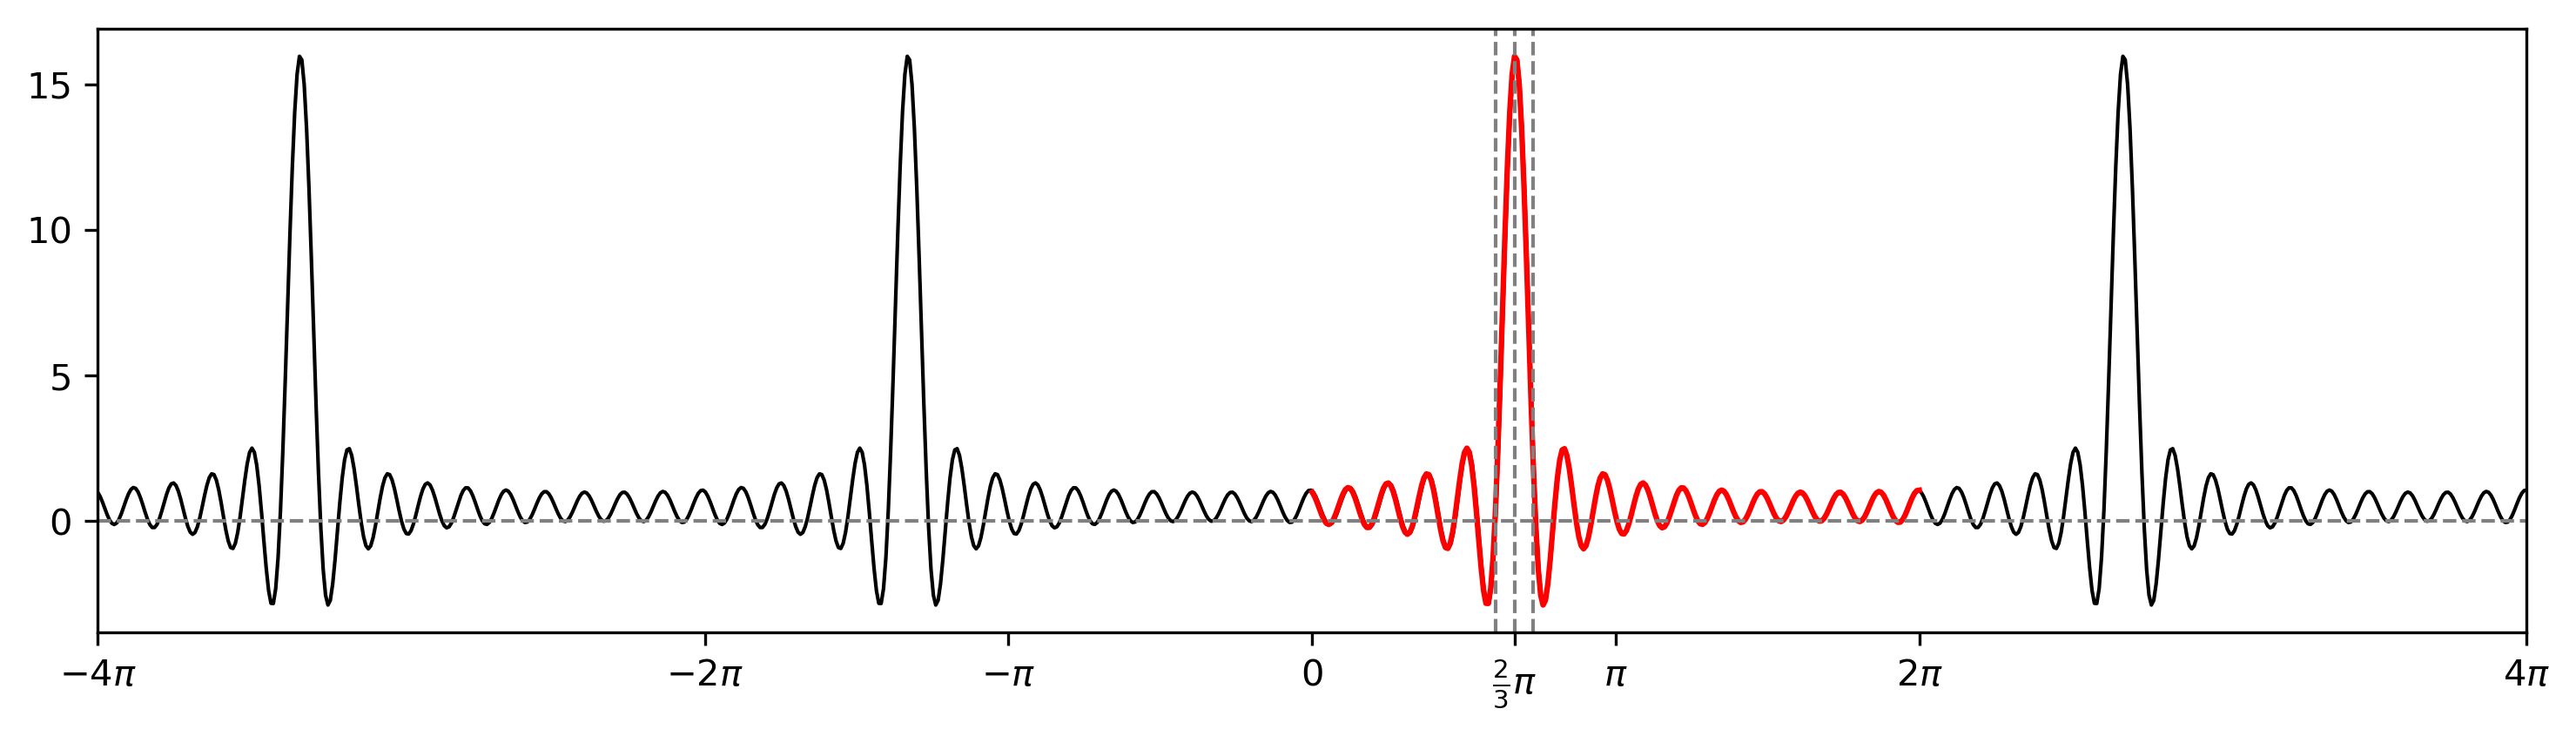
\includegraphics[width=6in]{external_image.png} 
    \fi
    \caption{Figure From File}
    \label{fig:fromfile}
\end{figure}


\end{homeworkProblem}


%%%%%%%%%%%%%%%%%%%%%%%%%%%%%%%%%%%%%%%%%%%%%%%%%%%%
%%%%%%%%%%%%%%%%%%%%%%%%%%%%%%%%%%%%%%%%%%%%%%%%%%%%
%%%%%%%%%%%%%%%%%%%%%%%%%%%%%%%%%%%%%%%%%%%%%%%%%%%%
%%%%%%%%%%%%%%%%%%%%%%%%%%%%%%%%%%%%%%%%%%%%%%%%%%%%
    
\begin{homeworkProblem}[1.2]
    An example of tabular data: \tref{tab:arrive}

    \begin{table}[H]
    \ifx \skipfigures \defined
    \begin{center}
    \begin{tabular}{l r}
    Sensor  & Arrival Time (ms) \\
    \hline
    0 & 4.50 \\
    1 & 4.25 \\
    2 & 4.00 \\
    3 & 3.75
    \end{tabular}
    \end{center}
    \fi
    \caption{Arrival Times}
    \label{tab:arrive}
    \end{table}


\end{homeworkProblem}
        
        
%%%%%%%%%%%%%%%%%%%%%%%%%%%%%%%%%%%%%%%%%%%%%%%%%%%%
%%%%%%%%%%%%%%%%%%%%%%%%%%%%%%%%%%%%%%%%%%%%%%%%%%%%
%%%%%%%%%%%%%%%%%%%%%%%%%%%%%%%%%%%%%%%%%%%%%%%%%%%%
%%%%%%%%%%%%%%%%%%%%%%%%%%%%%%%%%%%%%%%%%%%%%%%%%%%%

\begin{homeworkProblem}[1.3]

    Can include source code listings using the \code{lstlisting} package. \\
    \href{https://en.wikibooks.org/wiki/LaTeX/Source\_Code\_Listings}{\code{https://en.wikibooks.org/wiki/LaTeX/Source\_Code\_Listings}}

    The code can be written inline.
    \begin{lstlisting}[language=Python]
import numpy as np
180.0*np.arccos(0.1)/np.pi
    \end{lstlisting}

    Or included from an external file as in \lref{lst:external_example}.
    \lstinputlisting[language=Matlab, caption = {External File}, label=lst:external_example]{./external_file.m}

\end{homeworkProblem}

%%%%%%%%%%%%%%%%%%%%%%%%%%%%%%%%%%%%%%%%%%%%%%%%%%%%
%%%%%%%%%%%%%%%%%%%%%%%%%%%%%%%%%%%%%%%%%%%%%%%%%%%%
%%%%%%%%%%%%%%%%%%%%%%%%%%%%%%%%%%%%%%%%%%%%%%%%%%%%
%%%%%%%%%%%%%%%%%%%%%%%%%%%%%%%%%%%%%%%%%%%%%%%%%%%%

\begin{homeworkProblem}[1.5]
    \subsection{a)}
    An example of doing piece-wise expressions.
    \small
    \begin{align}
        \df{x_{1}} &= \begin{cases}
            1 & 0 \leq n \leq N-1 \\
            0 & otherwise
        \end{cases}
    \end{align}
    \normalsize
    
    \subsection{another subsection}
    Example of step by step derivation with explanation text.
    \small
    \begin{align}
        \ejO{X_{1}} &= \sum\limits_{n=0}^{N-1}e^{-j\Omega n} \\
        &= \frac{1-e^{-j\Omega N}}{1-e^{-j\Omega}} && \text{First N terms in geometric series} \\
        &= \frac{e^{-j\frac{\Omega N}{2}}\left[e^{j\frac{\Omega N}{2}}-e^{-j\frac{\Omega N}{2}}\right]\cdot2j}{e^{-j\frac{\Omega}{2}}\left[e^{j\frac{\Omega}{2}}-e^{-j\frac{\Omega}{2}}\right]\cdot2j} \\
        &= e^{-j\frac{\Omega N}{2}+\frac{\Omega}{2}}\frac{\sin\left(\frac{\Omega N}{2}\right)}{\sin\left(\frac{\Omega}{2}\right)} \\
        &= \frac{\sin\left(\frac{\Omega N}{2}\right)}{\sin\left(\frac{\Omega}{2}\right)}e^{-j\frac{\Omega}{2}\left(N-1\right)}
    \end{align}
    \normalsize

\end{homeworkProblem}
        
        
%%%%%%%%%%%%%%%%%%%%%%%%%%%%%%%%%%%%%%%%%%%%%%%%%%%%
%%%%%%%%%%%%%%%%%%%%%%%%%%%%%%%%%%%%%%%%%%%%%%%%%%%%
%%%%%%%%%%%%%%%%%%%%%%%%%%%%%%%%%%%%%%%%%%%%%%%%%%%%
%%%%%%%%%%%%%%%%%%%%%%%%%%%%%%%%%%%%%%%%%%%%%%%%%%%%

% Problem titles don't have to be numeric
\begin{homeworkProblem}[TWENTY]
    Some examples of helper commands for DSP expressions that I defined to reduce typing. (Plus an example of a footnote)
    \small
    \begin{align}
        \z{X} &= \cdots && \text{Z-transforms} \\
        \ejw{H} &= \cdots && \text{DTFT} \\
        \ejO{Y} &= \cdots && \text{DTFT with $\Omega$ instead of $\omega$} \\
        \nz{5} &= \cdots && \text{z to some power} \\
        \ejp{2\pi} &= \cdots && \text{positive powers of $e^{j}$} \\
        \ejn{2\pi} &= \cdots && \text{negative powers of $e^{j}$} \\
        \piover{2}{3} &= \cdots && \text{quick way to write fractions of $\pi$} \\
        \df{x} &= \cdots && \text{discrete signals} \\
        \dfd{x}{2} &= \cdots && \text{time shifted discrete signals} \\
        \dfn{x}{k} &= \cdots && \text{discrete signal with choice of index letter} \footnotemark
    \end{align}
    \normalsize
    \footnotetext{The code that defines these are in the preamble before the document begins. They are created using \code{newcommand}}

\end{homeworkProblem}
        
%%%%%%%%%%%%%%%%%%%%%%%%%%%%%%%%%%%%%%%%%%%%%%%%%%%%
%%%%%%%%%%%%%%%%%%%%%%%%%%%%%%%%%%%%%%%%%%%%%%%%%%%%
%%%%%%%%%%%%%%%%%%%%%%%%%%%%%%%%%%%%%%%%%%%%%%%%%%%%
%%%%%%%%%%%%%%%%%%%%%%%%%%%%%%%%%%%%%%%%%%%%%%%%%%%%

\begin{homeworkProblem}[5]
    Example of how to write a matrix
    \small
    \begin{align}
        \mtx{M}_{toeplitz} &= \begin{bmatrix}
        m_{0} & m_{-1} & m_{-2} & \cdots & m_{-n} \\
        m_{1} & m_{0} & m_{1} & \cdots & m_{-(n-1)} \\
        m_{2} & m_{1} & m_{0} & \cdots & m_{-(n-2)} \\
        \vdots & \vdots & \vdots & \ddots & \vdots \\
        m_{n} & m_{n-1} & m_{n-2} & \hdots & m_{0}
    \end{bmatrix} \label{eq:mtx}
    \end{align}
    \normalsize
    There are macros defined for many vector and matrix notations: $\mtx{a}$, $\mtxc{b}, \mtxt{A}, \mtxh{B}$. Use the base \code{mtx} macro with subscript and superscript for more complicated expressions such as $\mtx{A}_{i}^{-2H}$.
\end{homeworkProblem}

%%%%%%%%%%%%%%%%%%%%%%%%%%%%%%%%%%%%%%%%%%%%%%%%%%%%
%%%%%%%%%%%%%%%%%%%%%%%%%%%%%%%%%%%%%%%%%%%%%%%%%%%%
%%%%%%%%%%%%%%%%%%%%%%%%%%%%%%%%%%%%%%%%%%%%%%%%%%%%
%%%%%%%%%%%%%%%%%%%%%%%%%%%%%%%%%%%%%%%%%%%%%%%%%%%%

\begin{homeworkProblem}[6]
    Probability helpers
    \small
    \begin{align}
        \E{\frac{X}{Y}} &= \cdots && \text{Expected value using the proper capital E font} \\
        \Var{Z} &= \cdots && \text{Variance} \\
        x &\clsfr{b}{a} y && \text{Custom operator for bayes classifiers}
    \end{align}
    \normalsize
\end{homeworkProblem}

\section{Inter-Document Reference Helpers}
There are several macros defined to make consistent references with less redundant typing. For figures use \code{\textbackslash{}fref$\{label\}$} which will make all references to figure look like this - "\fref{fig:multi}". For tables use \code{\textbackslash{}tref$\{label\}$} for references that look like - "\tref{tab:arrive}". For equations use \code{\textbackslash{}eref$\{label\}$} for "\eref{eq:mtx}". And for code or unformatted text listings use \code{\textbackslash{}lref$\{label\}$} to get this - "\lref{lst:external_example}". Note that these generate clickable links.

\section{Using A Bibliography}
Just create a \code{.bib} file that contains bibtex entries and then reference them using \code{cite}. An example is \code{\textbackslash{}cite\{OpWill\}} which generates "\cite{OpWill}" because there is an entry in the included \code{.bib} file with label "OpWill". If you issue at least one \code{\textbackslash{}cite} command somewhere in your document then a "References" section as can be seen below will be added wherever the \code{\textbackslash{}bibliography} command was issued. You can change the citation style using \code{\textbackslash{}bibliographystyle}. Here I am using Alpha style.


\bibliographystyle{alpha}
\bibliography{tex_hw_bibliography.bib}

\end{document}
